\documentclass{beamer}[10]

\usepackage{graphicx}
\usepackage{xcolor}
\usepackage{tabto}
%\usepackage{beamerthemesplit}
\usepackage{tikz}
\usepackage{cancel}
\usepackage{verbatim}
\usepackage{fancybox}
\usepackage{enumerate}
\usepackage{amsmath,amssymb,amsthm,textcomp,mathtools}
\usepackage[super]{nth}
\usepackage[amssymb]{SIunits}
\usepackage{booktabs}
\usepackage{cancel}
\usepackage{bm}
\usepackage[utf8]{inputenc}
\usepackage{tabularx}
\usepackage{ragged2e}
\newcolumntype{Y}{ >{\RaggedRight\arraybackslash}X}
\usetikzlibrary{arrows,shapes}
\newcommand\T{\rule{0pt}{2.6ex}}
\newcommand\B{\rule[-1.2ex]{0pt}{0pt}}
\definecolor{UUcrimson}{RGB}{204,0,0}
\mode<presentation>
{ \usetheme{default}
  \usecolortheme[named=UUcrimson]{structure}
  \useinnertheme{circles}
  \setbeamercovered{transparent}
  \setbeamertemplate{blocks}[rounded]
  \usefonttheme[onlymath]{serif}
  \setbeamertemplate{navigation symbols}{}
  \setbeamertemplate{footline}[page number]
  \setbeamertemplate{navigation symbols}{}
  \setbeamercolor{section in toc}{fg=black,bg=white}
  \setbeamercolor{alerted text}{fg=UUcrimson!80!gray}
  \setbeamercolor*{palette primary}{fg=white,bg=UUcrimson}
  \setbeamercolor*{palette secondary}{fg=UUcrimson!70!black,bg=gray!15!white}
  \setbeamercolor*{palette tertiary}{bg=UUcrimson!80!black,fg=gray!10!white}
  \setbeamercolor*{palette quaternary}{fg=UUcrimson,bg=gray!5!white}
  \setbeamercolor*{palette sidebar primary}{fg=UUcrimson!10!black}
  \setbeamercolor*{palette sidebar secondary}{fg=white}
  \setbeamercolor*{palette sidebar tertiary}{fg=UUcrimson!50!black}
  \setbeamercolor*{palette sidebar quaternary}{fg=gray!10!white}
  \setbeamercolor{titlelike}{parent=palette primary,fg=white}
  \setbeamercolor{frametitle}{bg=UUcrimson}
  \setbeamercolor{frametitle right}{bg=UUcrimson}
  \setbeamercolor*{separation line}{}
  \setbeamercolor*{fine separation line}{}
}

\usetikzlibrary{backgrounds}
\makeatletter
\tikzstyle{every picture}+=[remember picture]
\tikzset{%
  fancy quotes/.style={
    text width=\fq@width pt,
    align=justify,
    inner sep=1em,
    anchor=north west,
    minimum width=\linewidth,
    font=\itshape
  },
  fancy quotes width/.initial={.8\linewidth},
  fancy quotes marks/.style={
    scale=8,
    text=white,
    inner sep=0pt,
  },
  fancy quotes opening/.style={
    fancy quotes marks,
  },
  fancy quotes closing/.style={
    fancy quotes marks,
  },
  fancy quotes background/.style={
    show background rectangle,
    inner frame xsep=0pt,
    background rectangle/.style={
      fill=gray!25,
      rounded corners,
    },
  }
}
\newenvironment{fancyquotes}[1][]{%
\noindent
\tikzpicture[fancy quotes background]
\node[fancy quotes opening,anchor=north west] (fq@ul) at (0,0) {``};
\tikz@scan@one@point\pgfutil@firstofone(fq@ul.east)
\pgfmathsetmacro{\fq@width}{\linewidth - 2*\pgf@x}
\node[fancy quotes,#1] (fq@txt) at (fq@ul.north west) \bgroup}
{\egroup;
\node[overlay,fancy quotes closing,anchor=east] at (fq@txt.south east) {''};
\endtikzpicture}
\makeatother


\usetikzlibrary{backgrounds}
\makeatletter
\tikzstyle{every picture}+=[remember picture]
\tikzset{%
  fancy defs/.style={
    text width=\fq@width pt,
    align=justify,
    inner sep=0.25em,
    anchor=north west,
    minimum width=\linewidth,
    font=\itshape
  },
  fancy defs width/.initial={.8\linewidth},
  fancy defs marks/.style={
    scale=8,
    text=white,
    inner sep=0pt,
  },
  fancy defs opening/.style={
    fancy defs marks,
  },
  fancy defs closing/.style={
    fancy defs marks,
  },
  fancy defs background/.style={
    show background rectangle,
    inner frame xsep=0pt,
    background rectangle/.style={
      fill=gray!25,
      rounded corners,
    },
  }
}
\newenvironment{fancydefs}[1][]{%
\noindent
\tikzpicture[fancy defs background]
\node[fancy defs opening,anchor=north west] (fq@ul) at (0,0) {};
\tikz@scan@one@point\pgfutil@firstofone(fq@ul.east)
\pgfmathsetmacro{\fq@width}{\linewidth - 2*\pgf@x}
\node[fancy defs,#1] (fq@txt) at (fq@ul.north west) \bgroup}
{\egroup;
\node[overlay,fancy defs closing,anchor=east] at (fq@txt.south east) {};
\endtikzpicture}
\makeatother
\usepackage{scalerel}[2014/03/10]
\usepackage{stackengine}
\usepackage{empheq}
\newcommand*\widefbox[1]{\fbox{\hspace{0.5em}#1\hspace{0.5em}}}

\newcommand\reallywidetilde[1]{\ThisStyle{%
  \setbox0=\hbox{$\SavedStyle#1$}%
  \stackengine{-.1\LMpt}{$\SavedStyle#1$}{%
    \stretchto{\scaleto{\SavedStyle\mkern.2mu\sim}{.5467\wd0}}{.4\ht0}%
%    .2mu is the kern imbalance when clipping white space
%    .5467++++ is \ht/[kerned \wd] aspect ratio for \sim glyph
  }{O}{c}{F}{T}{S}%
}}
\usepackage{media9}

\logo{
\includegraphics[width=0.75cm]{logo.jpg}}
\author[Gibbs]{Dr. Jeremy A. Gibbs}
\institute{Department of Mechanical Engineering\\University of Utah}
\date{Spring 2017}
\title{Environmental Fluid Dynamics: Lecture 7}
% colors
\definecolor{colororange}{HTML}{E65100} % orange
\definecolor{colordgray}{HTML}{795548} % dark gray for note
\definecolor{colorhgray}{HTML}{212121} % heavy dark gray for normal text
\definecolor{colorgreen}{HTML}{009688} % green
\definecolor{colorwhite}{HTML}{FFFFFF} % background white
\definecolor{colorlgray}{HTML}{F5F3EE} % background light gray
\definecolor{colorblue}{HTML}{0277BB} % blue
\definecolor{colorred}{HTML}{CC0000} % red
\newcommand{\fontsizeone}{1.9em}
\setbeamertemplate{caption}{\raggedright\insertcaption\par}
\newcommand{\framecard}[2][colorgreen]{
  {\setbeamercolor{background canvas}{bg=#1}
    \begin{frame}[plain]
    \vfill
    \begin{center}
     {#2}
    \end{center}
    \vfill
    \end{frame}
  }
}
\begin{document}

%----------------------------------------------------------------------------------------
%	TITLE & TOC SLIDES
%----------------------------------------------------------------------------------------

\begin{frame} 
  \titlepage
\end{frame}

%------------------------------------------------

\begin{frame}
\frametitle{Overview}
\tableofcontents
\end{frame}

%------------------------------------------------
\section{Atmospheric Thermodynamics: Evapotranspiration} %
%------------------------------------------------
\framecard[colorred]{{\color{white}\Huge Atmospheric Thermodynamics:\\~\\Evapotranspiration}}
%------------------------------------------------
\subsection{Definition}
%------------------------------------------------

\begin{frame}{Atmospheric Thermodynamics: Evapotranspiration}

\textbf{Evaporation}
\begin{fancydefs}
	Conversion from liquid to vapor state
\end{fancydefs}

\begin{itemize}
	\item free water surface
	\item moist soil surface
	\item leaves of living plants $\Rightarrow$ transpiration
\end{itemize}
\end{frame}

%------------------------------------------------
\subsection{Physics}
%------------------------------------------------

\begin{frame}{Atmospheric Thermodynamics: Evapotranspiration}
\begin{itemize}
	\item Similar to molecular transfer of heat and momentum at a surface
	\item \textit{Mass transfer} - occurring within first few molecular path lengths of the surface
	\item \textbf{Fick's Law}
	\begin{fancydefs}
		The net flux of mass in a given direction is proportional to the concentration gradient in that direction
	\end{fancydefs}
\end{itemize}
\end{frame}
%------------------------------------------------

\begin{frame}{Atmospheric Thermodynamics: Evapotranspiration}
\textbf{Fick's Law}
\begin{itemize}
	\item The evaporation rate over a horizontal surface for a laminar flow is given by
	$$E_0 = -\rho \alpha_w\frac{\partial q}{\partial z}$$
	where
	\begin{itemize}
		\item $E_0$ [$\kilo\gram\ \metre\rpsquared\ \reciprocal\second$] is the evaporation rate
		\item $\rho$ [$\kilo\gram\ \metre\rpcubed$] is total density
		\item $\alpha_w$ [$\metre\squared\ \reciprocal\second$] is molecular diffusivity of water.
		\item $q$ is specific humidity\\~\\Typical values of $\alpha$ are
		\begin{align*}
			\alpha_w(0) &= 21.2\times10^{-6}\ \metre\squared\ \reciprocal\second\\
			\frac{\alpha(T)}{\alpha_w(0)} &= (1 + 0.007T) 
		\end{align*} 
	\end{itemize}
\end{itemize}
\end{frame}

%------------------------------------------------

\begin{frame}{Atmospheric Thermodynamics: Evapotranspiration}
\textbf{Turbulent flow}
\begin{itemize}
	\item mixing is dominated by ``eddy motion'' that is much more efficient
	\item phenomenological model
	$$E=-\rho K_w \frac{\partial \overline{q}}{\partial z}$$
	where
	\begin{itemize}
		\item $K_w$ is the turbulent transfer coefficient (``eddy diffusivity''), which is much greater in magnitude than its molecular counterpart ($\sim 0.1-1\ \metre\squared\ \reciprocal\second$)
		\item $K_w$ has limited applicability, is not constant (depends on $T$)
	\end{itemize}
\end{itemize}
\end{frame}

%------------------------------------------------

\begin{frame}{Atmospheric Thermodynamics: Evapotranspiration}
Consider a fully saturated soil surface, \textit{i.e.}, moisture content is no longer a limiting factor:\\
\textbf{Potential evaporation rate} $E_p$
\begin{fancydefs}
	the maximum rate of evaporation for a given surface under a set of meteorological conditions
\end{fancydefs}

For a unsaturated soil surface:\\
\textbf{Actual evaporation rate} depends on
\begin{itemize}
	\item $T_S$
	\item turbulence: near-surface wind speed
	\item specific humidity
	\item stability
	\item plant physiology
	\item moisture content of soil
\end{itemize}
\end{frame}

%------------------------------------------------
\subsection{Methods of Determination}
%------------------------------------------------

\begin{frame}{Methods for Determining: Direct Measurement}
\textbf{Lysimeter}
\begin{columns}[T]
    \begin{column}{.4\textwidth}
    \begin{minipage}[c][0.7\textheight][c]{\linewidth}
    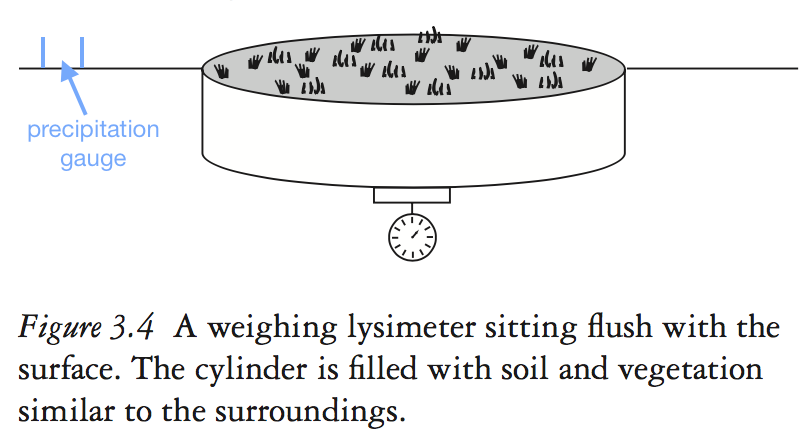
\includegraphics[width=1\textwidth]{fig1}\\
    \centering \small From Davie (2008)
    \end{minipage}
    \end{column}
    \begin{column}{.6\textwidth}
    \begin{minipage}[c][0.6\textheight][c]{\linewidth}
   \begin{itemize}
   	\item Water mass balance on the soil
   	$$P = E + \Delta r + \Delta s$$
   	where 
   	\begin{itemize}
   	\item $P$ is precipitation
   	\item $E$ is evapotranspiration
   	\item $\Delta r$ is runoff
   	\item $\Delta s$ is storage
   	\end{itemize}
   	\item Most have $\sim 1$-$6\ \metre$ diameter and $1$-$2\ \metre$ depth 
   	\item Basically, the change in storage of water is modeled by the change in weight of the soil
   \end{itemize}
      \end{minipage}
    \end{column}
  \end{columns}
\end{frame}

%------------------------------------------------

\begin{frame}{Methods for Determining: Direct Measurement}
\textbf{Evaporation Pan}
\begin{columns}[T]
    \begin{column}{.4\textwidth}
    \begin{minipage}[c][0.7\textheight][c]{\linewidth}
    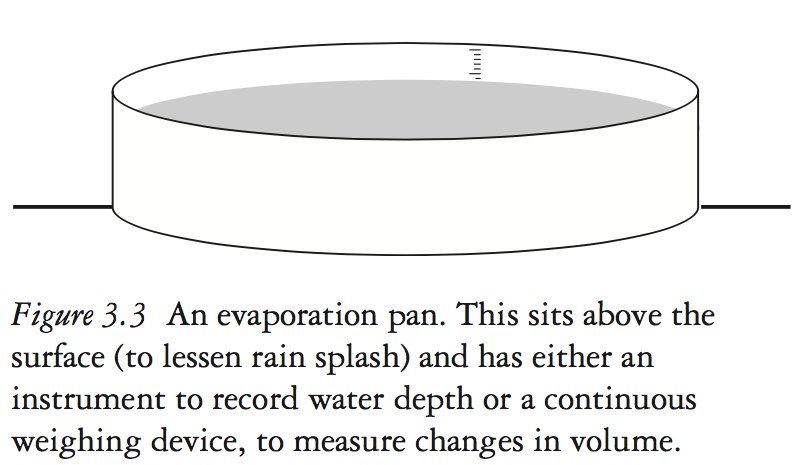
\includegraphics[width=1\textwidth]{fig2}\\
    \centering \small From Davie (2008)
    \end{minipage}
    \end{column}
    \begin{column}{.6\textwidth}
    \begin{minipage}[c][0.6\textheight][c]{\linewidth}
   \begin{itemize}
   	\item Cylindrical pans ($1$-$5\ \metre$ diameter, $0.25$-$1\ \metre$ depth)
   	\item Measures free-water evaporation $E_0$ by monitoring water-level change in the pan
   	\item $E_0$ is generally larger than $E_t$ because evaporation in a catchment occurs over land where available water is in soil and potentially limited
   	\item More appropriate for estimating water loss from lakes, ponds, and reservoirs
   \end{itemize}
      \end{minipage}
    \end{column}
  \end{columns}
\end{frame}

%------------------------------------------------

\begin{frame}{Methods for Determining: Direct Measurement}
\textbf{Eddy Covariance}
\begin{columns}[T]
    \begin{column}{.4\textwidth}
    \begin{minipage}[c][0.7\textheight][c]{\linewidth}
    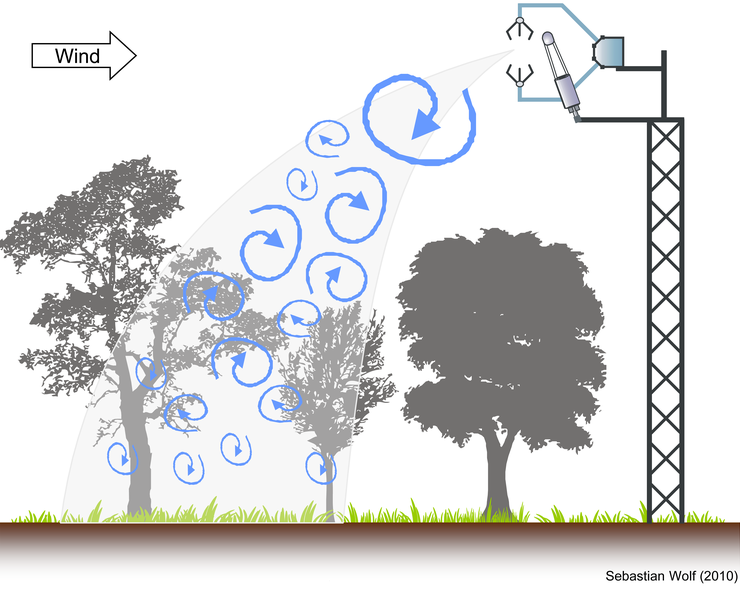
\includegraphics[width=1\textwidth]{fig3}\\
    \centering \small From Wolfe (2010)
    \end{minipage}
    \end{column}
    \begin{column}{.6\textwidth}
    \begin{minipage}[c][0.6\textheight][c]{\linewidth}
   \begin{itemize}
   	\item Measures vertical transport of water vapor driven by convective motion with a sonic anemometer + IRGA or open path hygrometer
   	\item Flux is instantaneously determined by sensing the properties of eddies as they pass through the sensor
   	$$E = \rho \overline{w^\prime q^\prime}$$
   	where the bar is the average over some specified temporal window
   	\item Let's relate these fluxes to gradients
   \end{itemize}
      \end{minipage}
    \end{column}
  \end{columns}
\end{frame}

%------------------------------------------------

\begin{frame}{Methods for Determining: Direct Measurement}
\textbf{Eddy Covariance}
\begin{columns}[T]
    \begin{column}{.4\textwidth}
    \begin{minipage}[c][0.7\textheight][c]{\linewidth}
    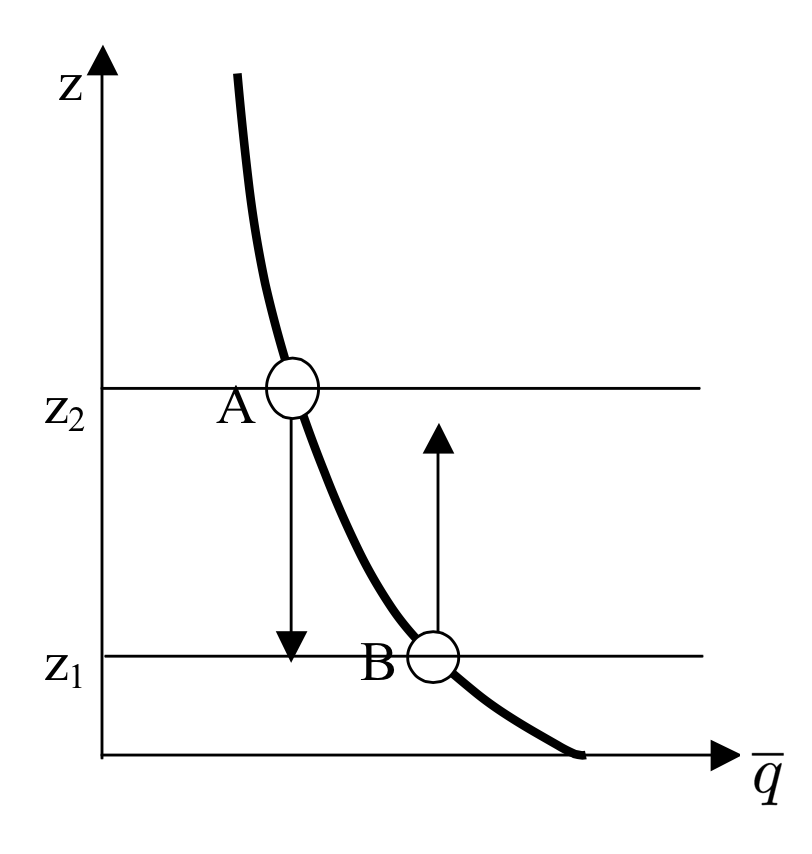
\includegraphics[width=1\textwidth]{fig4}\\
    \centering \small From Wolfe (2010)
    \end{minipage}
    \end{column}
    \begin{column}{.6\textwidth}
    \begin{minipage}[c][0.6\textheight][c]{\linewidth}
   \begin{itemize}
   	\item Specific humidity usually decreases with height
   	\item Imagine parcel A is moved down, and parcel B is moved up, by some eddy
   	\item For parcel A
   	$$w^\prime <0,\ q^\prime < 0,\ w^\prime q^\prime>0$$
   	\item For parcel B
   	$$w^\prime >0,\ q^\prime > 0,\ w^\prime q^\prime>0$$
   \end{itemize}
      \end{minipage}
    \end{column}
  \end{columns}
\end{frame}

%------------------------------------------------

\begin{frame}{Methods for Determining: Direct Measurement}
\textbf{Scintillometry}
\begin{itemize}
	\item Uses the concept that there are large variations of the index of refraction in the atmosphere that result from turbulent eddy motion
	\item Measures radiation intensity fluctuations from the laser source that result from humidity and temperature variations
\end{itemize}
\begin{figure}
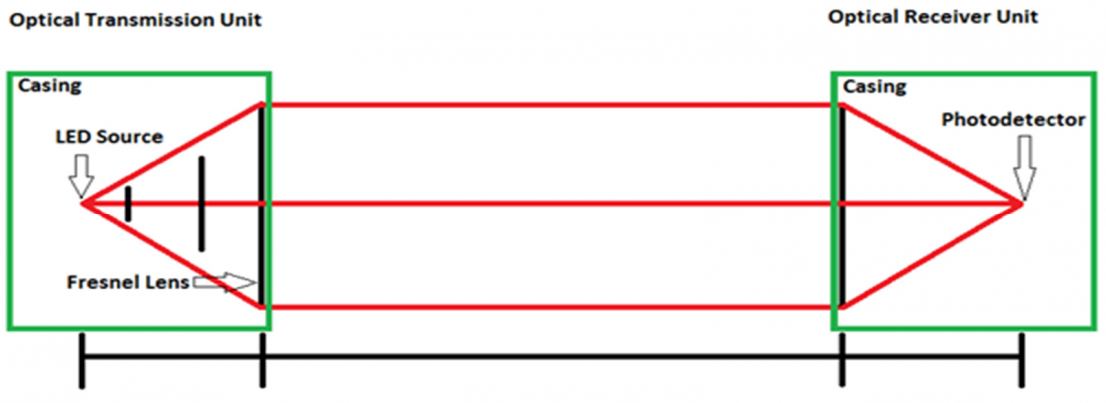
\includegraphics[width=0.7\textwidth]{fig5}	
\end{figure}
\end{frame}

%------------------------------------------------

\begin{frame}{Methods for Determining: Direct Measurement}
\textbf{Scintillometry}
\begin{itemize}
	\item Structure function
	$$D_n (\vec{r}) = \overline{[n(\vec{x}) - n(\vec{x} + \vec{r}]^2}$$
	where $\vec{r}$ is a separation vector
	\item We can relate $D_n$ to a constant called the structure parameter $C_n^2$:
	$$C_n^2 = D_n/r^{(2/3)}$$
	where $r=|\vec{r}|$.
	\item This can further be related to $C_T^2$ and $C_q^2$ (more later in the course)
\end{itemize}
\end{frame}

%------------------------------------------------

\begin{frame}{Methods for Determining: Direct Measurement}
\textbf{Scintillometry}
\begin{itemize}
	\item The intensity $I \propto C_n^2$
	\item Optical wavelengths (visible-near IR): $C_n^2 \rightarrow C_T^2$
	\item Radio wavelength (using RWS, expensive): $C_n^2 \rightarrow C_q^2$
	\item These can be used to determine $H_S$ and $H_L$ using Monin-Obukhov Similarity Theory (MOST), which implies that MOST is satisfied in the surface layer
	\item In this sense, the scintillometer approach is less direct since we obtain fluxes through empirical expressions
\end{itemize}
\end{frame}

%------------------------------------------------

\begin{frame}{Methods for Determining: Direct Measurement}
\textbf{Scintillometry}
\begin{itemize}
	\item The Fresnel Length ($F=\sqrt{\lambda L}$) is a measure of the size of the most active eddy in a signal
	\item Small Aperture Scintillometers (SAS) are usually operated from $50\ \metre$ to $500\ \metre$
	\item Large Aperture Scintillometers (LAS) are usually operated from $500\ \metre$ to $5\ \kilo\metre$
	\item We get a spatial average, whereas other methods give point measurements
\end{itemize}
\end{frame}
%------------------------------------------------

\begin{frame}{Methods for Determining: Energy Balance/Bowen Ratio}
\textbf{Energy Balance/Bowen Ratio}
$$E_0 = \frac{H_L}{L_v}$$
where we showed already that
\begin{align*}
H_S &= \frac{R_N - H_G}{1+B^{-1}}\\
H_L &= \frac{R_N - H_G}{1+B}
\end{align*}
and
$$B=\frac{H_S}{H_L} \approx \underbrace{\frac{\rho c_p K_H\cfrac{\partial \overline{\theta}}{\partial z}}{\rho L_v K_q \cfrac{\partial \overline{q}}{\partial z}}}_{K_H \sim K_q} \approx \frac{c_p}{L_v}\frac{\Delta \theta}{\Delta q}$$
\end{frame}

%------------------------------------------------

\begin{frame}{Methods for Determining: Bulk Transfer Approach}
\textbf{Bulk Transfer Approach}
\begin{itemize}
	\item The bulk transfer formula for water vapor flux is
	\begin{align*}
	E_0 &= \rho C_w U_r (q_0 - q_r)\\
	H_0 &= \rho c_p C_H (\theta_0 - \theta_r)
	\end{align*}
	where
	\begin{itemize}
		\item $C_w, C_H$ are the bulk transfer coefficients for water vapor and heat
		\item $U_r$ is velocity at some reference level
		\item $q_0, \theta_0$ are specific humidity and temperature at roughness height $z_0$
		\item $q_r, \theta_r$ are specific humidity and temperature at some reference level
	\end{itemize}
	\item Requires measurement of wind speed, temperature, and specific humidity
	\begin{itemize}
		\item $q_0$ and $\theta_0$ are very tough to measure at $z_0$
	\end{itemize}
\end{itemize}
\end{frame}

%------------------------------------------------

\begin{frame}{Methods for Determining: Bulk Transfer Approach}
\textbf{Bulk Transfer Approach}
\begin{itemize}
	\item Alternative form (usually good for water surfaces)
	\begin{align*}
	E_0 &= C_w U_r (q_s - q_r)\\
	H_0 &= \rho c_p C_H U_r (\theta_s-\theta_r)
	\end{align*}
	\item Since $z_o$ is so small for water surfaces, we can use surface values
	\item $\theta_s$ is available from satellite measurements
	\item $q_s$ is determined from the saturation value at $T_s$
	\item Note: for neutral conditions, $C_w, C_H\sim 1.2\times 10^{-3}$ (dependent on surface roughness, measurement height, and stability)
\end{itemize}
\end{frame}

%------------------------------------------------

\begin{frame}{Methods for Determining: Bulk Transfer Approach}
\textbf{Bulk Transfer Approach}
\begin{figure}
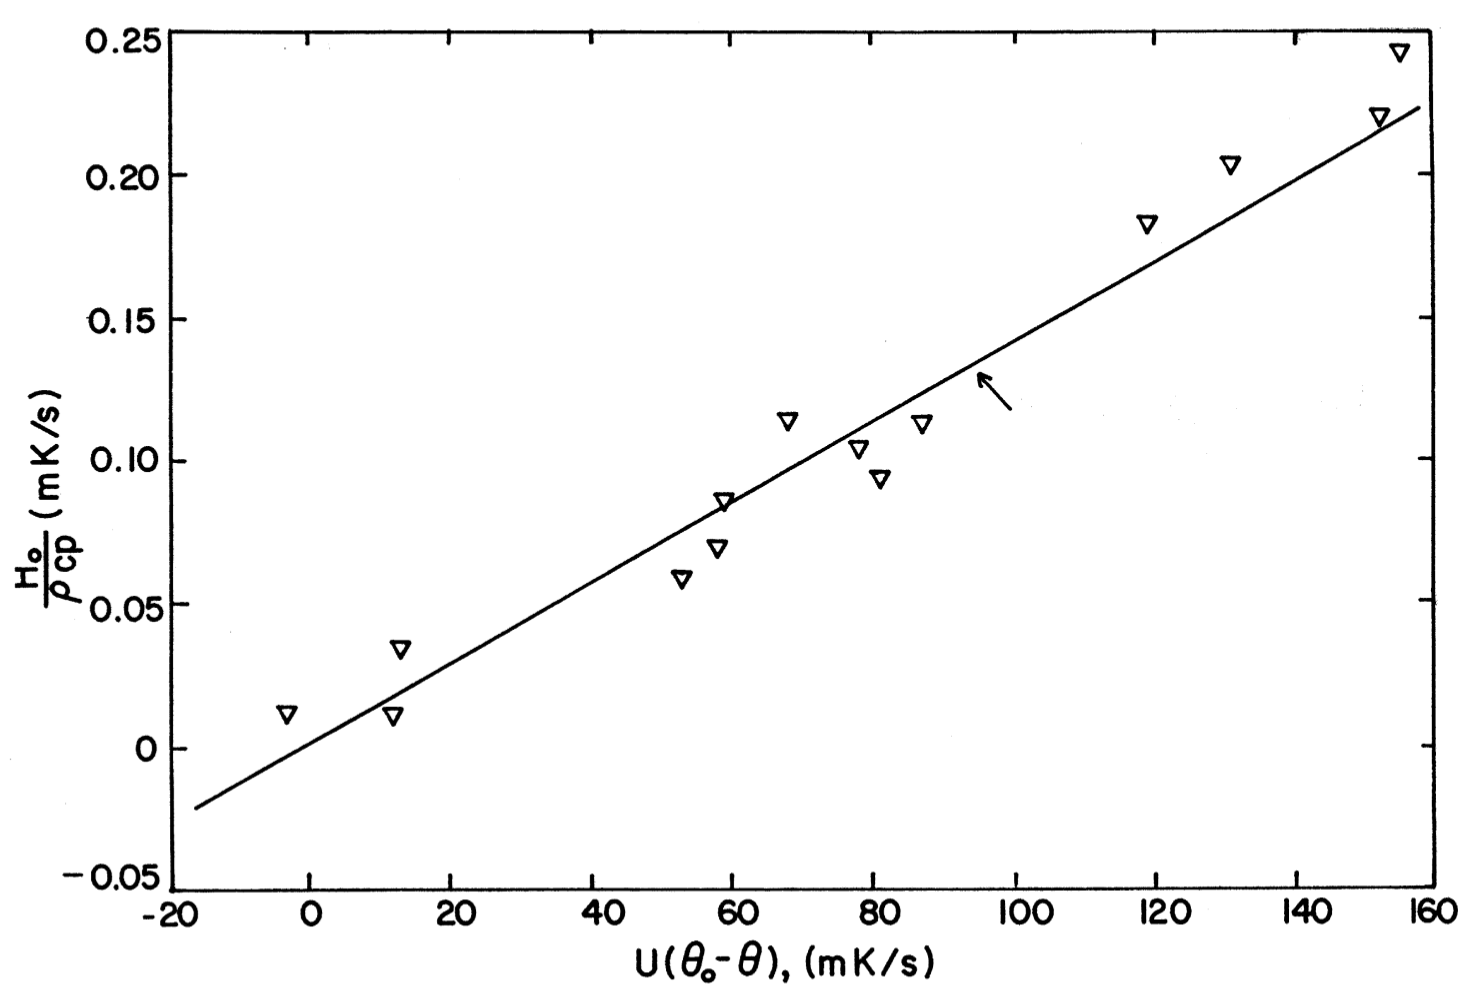
\includegraphics[width=0.485\textwidth]{fig6}
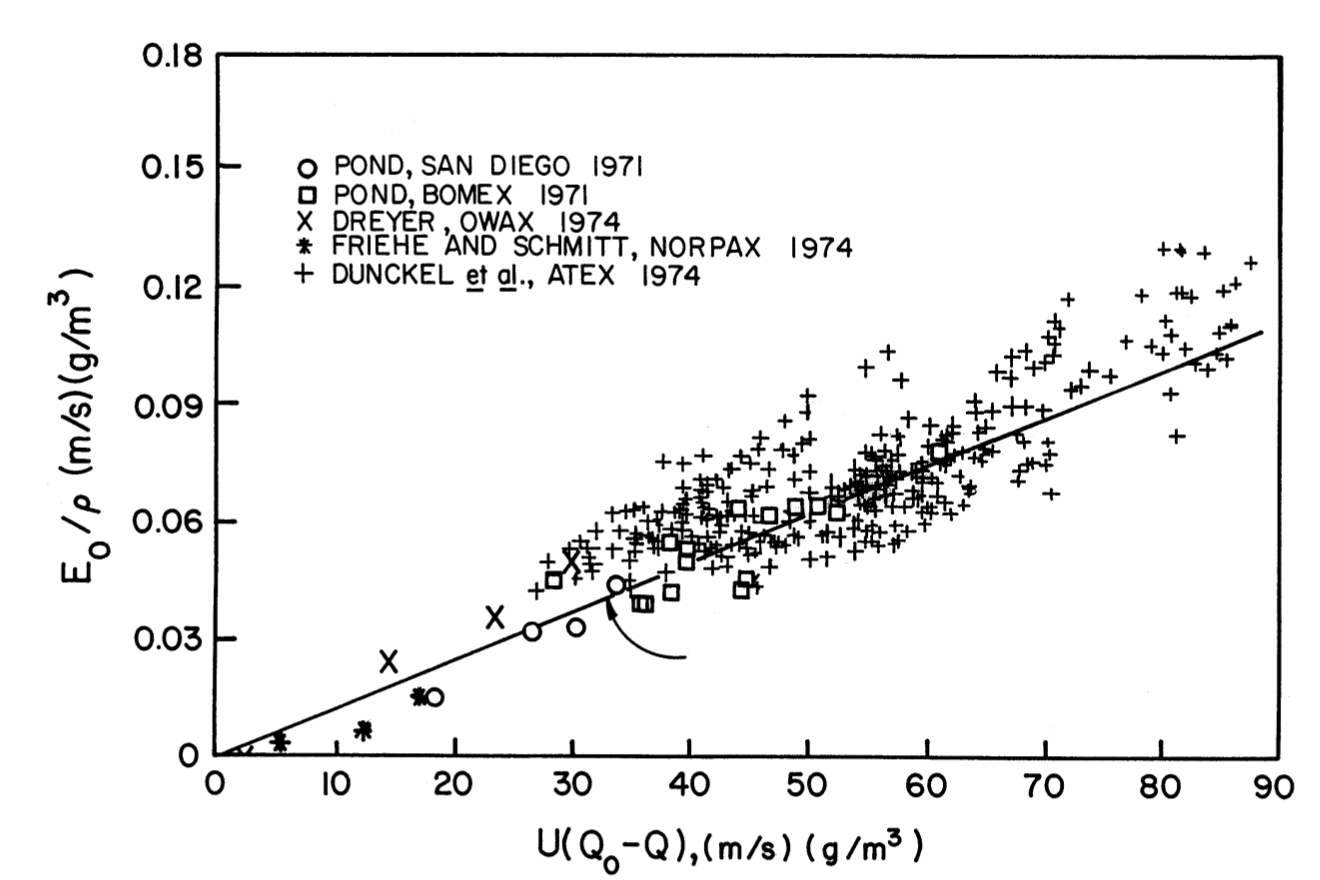
\includegraphics[width=0.515\textwidth]{fig7}
\centering \small From Arya (2001)
\end{figure}

\end{frame}

%------------------------------------------------

\begin{frame}{Methods for Determining: Penman Approach}
\textbf{Penman Approach}
\begin{itemize}
	\item A combination of energy balance and bulk transfer
	\item Penman (1948) derived a formula for evaporation over open water and saturated land
	\begin{align*}
	E_0 &= \rho C_w U_r(q_0 - q_r^*) + E_a\\
	E_a &= \rho C_w U_r(q_r* - q_r)\\
	H_0 &= \rho c_p C_H U_r(T_0 - T_r)
	\end{align*}
	where $q_r^*$ is the saturation specific humidity and $E_a$ is the ``drying power'' of air (related to advection)
\end{itemize}
\end{frame}

%------------------------------------------------

\begin{frame}{Methods for Determining: Penman Approach}
\textbf{Penman Approach}
\begin{itemize}
	\item If $C_w=C_H$
	\begin{align*}
	\frac{L_v E_0}{H_0} &= \frac{\cancelto{}{\rho} \cancelto{}{C_w} L_v \cancelto{}{U_r}(q_0 - q_r^*)}{\cancelto{}{\rho} c_p \cancelto{}{C_H} \cancelto{}{U_r}(T_0 - T_r)} + \frac{L_v E_0}{H_0}\\
	\frac{L_v E_0}{H_0} &= \frac{L_v}{c_p} \frac{(q_0 - q_r^*)}{(T_0 - T_r)} + \frac{L_v E_0}{H_0} = \text{BR}^{-1}
	\end{align*}
	Recall, $q = 0.622 e/p$ - so
	$$\text{BR}^{-1} = \underbrace{\frac{0.622}{c_p}\frac{L_v}{p}}_{I} \underbrace{\frac{(e_0 - e_r^*)}{(T_0 - T_r)}}_{II} + \text{BR}^{-1}\frac{E_a}{E_0}$$
\end{itemize}
\end{frame}

%------------------------------------------------

\begin{frame}{Methods for Determining: Penman Approach}
\textbf{Penman Approach}
$$\text{BR}^{-1} = \underbrace{\frac{0.622}{c_p}\frac{L_v}{p}}_{I} \underbrace{\frac{(e_0 - e_r^*)}{(T_0 - T_r)}}_{II} + \text{BR}^{-1}\frac{E_a}{E_0}$$
\begin{itemize}
	\item (I) $\gamma = \frac{c_p p}{0.622 L_v}$ = psychrometric constant
	\item (II) $\Delta = \frac{(e_0 - e_r^*)}{(T_0 - T_r)} \approx \frac{d e_s}{d_T}$, valid when $e_r^*$ is close to $e_0$ (i.e., a nearly saturated surface)
	\item Note: $\Delta$ is the slope of the saturation vapor pressure vs. temperature curve evaluated at $(T_0 + T_r)/2$
\end{itemize}
\end{frame}

%------------------------------------------------

\begin{frame}{Methods for Determining: Penman Approach}
\textbf{Penman Approach}
\begin{itemize}
	\item Thus, 
	\begin{align*}
	\text{BR}^{-1} &= \frac{\Delta}{\gamma} + \text{BR}^{-1}\frac{E_a}{e_0}\\
	\text{BR}(\frac{\Delta}{\gamma}) &= 1-\frac{E_a}{E_0} = \frac{E_0-E_a}{E_0}\\
	\Aboxed{\text{BR} &= \frac{\gamma}{\Delta}\left(\frac{E_0-E_a}{E_0}\right)}
	\end{align*}
	\item Recall from the energy equation that
	$$H_L = \frac{R_N - H_G}{1 + \text{BR}} = E_0 L_v$$
	such that 
	$$\text{BR} = \frac{R_N - H_G}{E_o L_v} -1$$ 
\end{itemize}
\end{frame}

%------------------------------------------------

\begin{frame}{Methods for Determining: Penman Approach}
\textbf{Penman Approach}
\begin{itemize}
	\item Equating yields
	\begin{align*}
	 \left[\frac{\gamma}{\Delta}\left(\frac{E_0-E_a}{E_0}\right)\right. &= \left.\frac{R_N - H_G}{E_o L_v} -1\right]E_0\\
\frac{\gamma}{\Delta}(E_0-E_a) &= \frac{R_N - H_G}{L_v} - E_0\\
   E_0\left(1+\frac{\gamma}{\Delta}\right) &= \frac{R_N - H_G}{L_v} + E_a\frac{\gamma}{\Delta}\\
\Aboxed{E_0 &= \frac{\Delta}{\gamma + \Delta} \frac{R_N - H_G}{L_v} + \underbrace{\frac{\gamma}{\gamma+\Delta}E_a}_{\text{III}}}
	\end{align*}
	where (III) is departure from equilibrium in the atmosphere
\end{itemize}
\end{frame}

%------------------------------------------------

\begin{frame}{Methods for Determining: Penman Approach}
\textbf{Penman Approach}
$$E_0 = \frac{\Delta}{\gamma + \Delta} \frac{R_N - H_G}{L_v} +\frac{\gamma}{\gamma+\Delta}E_a$$
\begin{itemize}
	\item Need to measure:
	\begin{itemize}
		\item soil heat flux
		\item net radiation
		\item temperature
		\item humidity
		\item wind speed
	\end{itemize}
	\item Do not need surface temperature!
\end{itemize}
\end{frame}
%------------------------------------------------

\begin{frame}{Methods for Determining: Penman Approach}
\textbf{Penman Approach}
$$E_0 = \frac{\Delta}{\gamma + \Delta} \frac{R_N - H_G}{L_v} +\frac{\gamma}{\gamma+\Delta}E_a$$
\begin{itemize}
	\item To simplify, note that for a wide, very wet surface $e\rightarrow e_s$
	$$E_0 = \frac{\Delta}{\gamma + \Delta} \frac{R_N - H_G}{L_v}$$
	this is called the equilibrium evapotranspiration
	\item Here, we only need to measure $T$ and estimate $R_N - H_G$
	\item If valid, it is implied that 
	$$\text{BR} = \frac{\gamma}{\Delta}$$
	\item Sensible heat flux ($E_a$ negligible)
	$$H_S \approx \frac{\gamma}{\gamma + \Delta}(R_N - H_G)$$
\end{itemize}
\end{frame}

%------------------------------------------------

\begin{frame}{Methods for Determining: Priestly-Taylor}
\textbf{Priestly-Taylor Modification}
\begin{align*}
H_L &\approx \frac{\Delta}{\Delta + \gamma} (R_N - H_G) \alpha_{pt}\\
H_S &\approx \frac{\gamma}{\gamma + \Delta}(R_N - H_G)(1-\alpha_{pt})
\end{align*}
where $\alpha_{pt}\sim 1.25$ for advection free conditions on a well waters surface (JAM,, 1982)

\end{frame}

%------------------------------------------------

\begin{frame}{Methods for Determining: de Bruin and Holtslag}
\textbf{de Bruin and Holtslag Modification}\\
Canopy with storage for non-saturated surface

\begin{align*}
H_L &\approx \alpha \frac{\Delta}{\Delta + \gamma} (R_N - \Delta H_s) + \beta\\
H_S &\approx (1-\alpha) \frac{\Delta}{\Delta + \gamma}(R_N - \Delta H_s) - \beta
\end{align*}
where $\alpha$ depends on moisture status
~\\~\\
This is almost identical to the LUMPS model (see paper)

\end{frame}

%------------------------------------------------

\begin{frame}{Methods for Determining: LUMPS Model}
\textbf{LUMPS Model}\\
\begin{figure}
	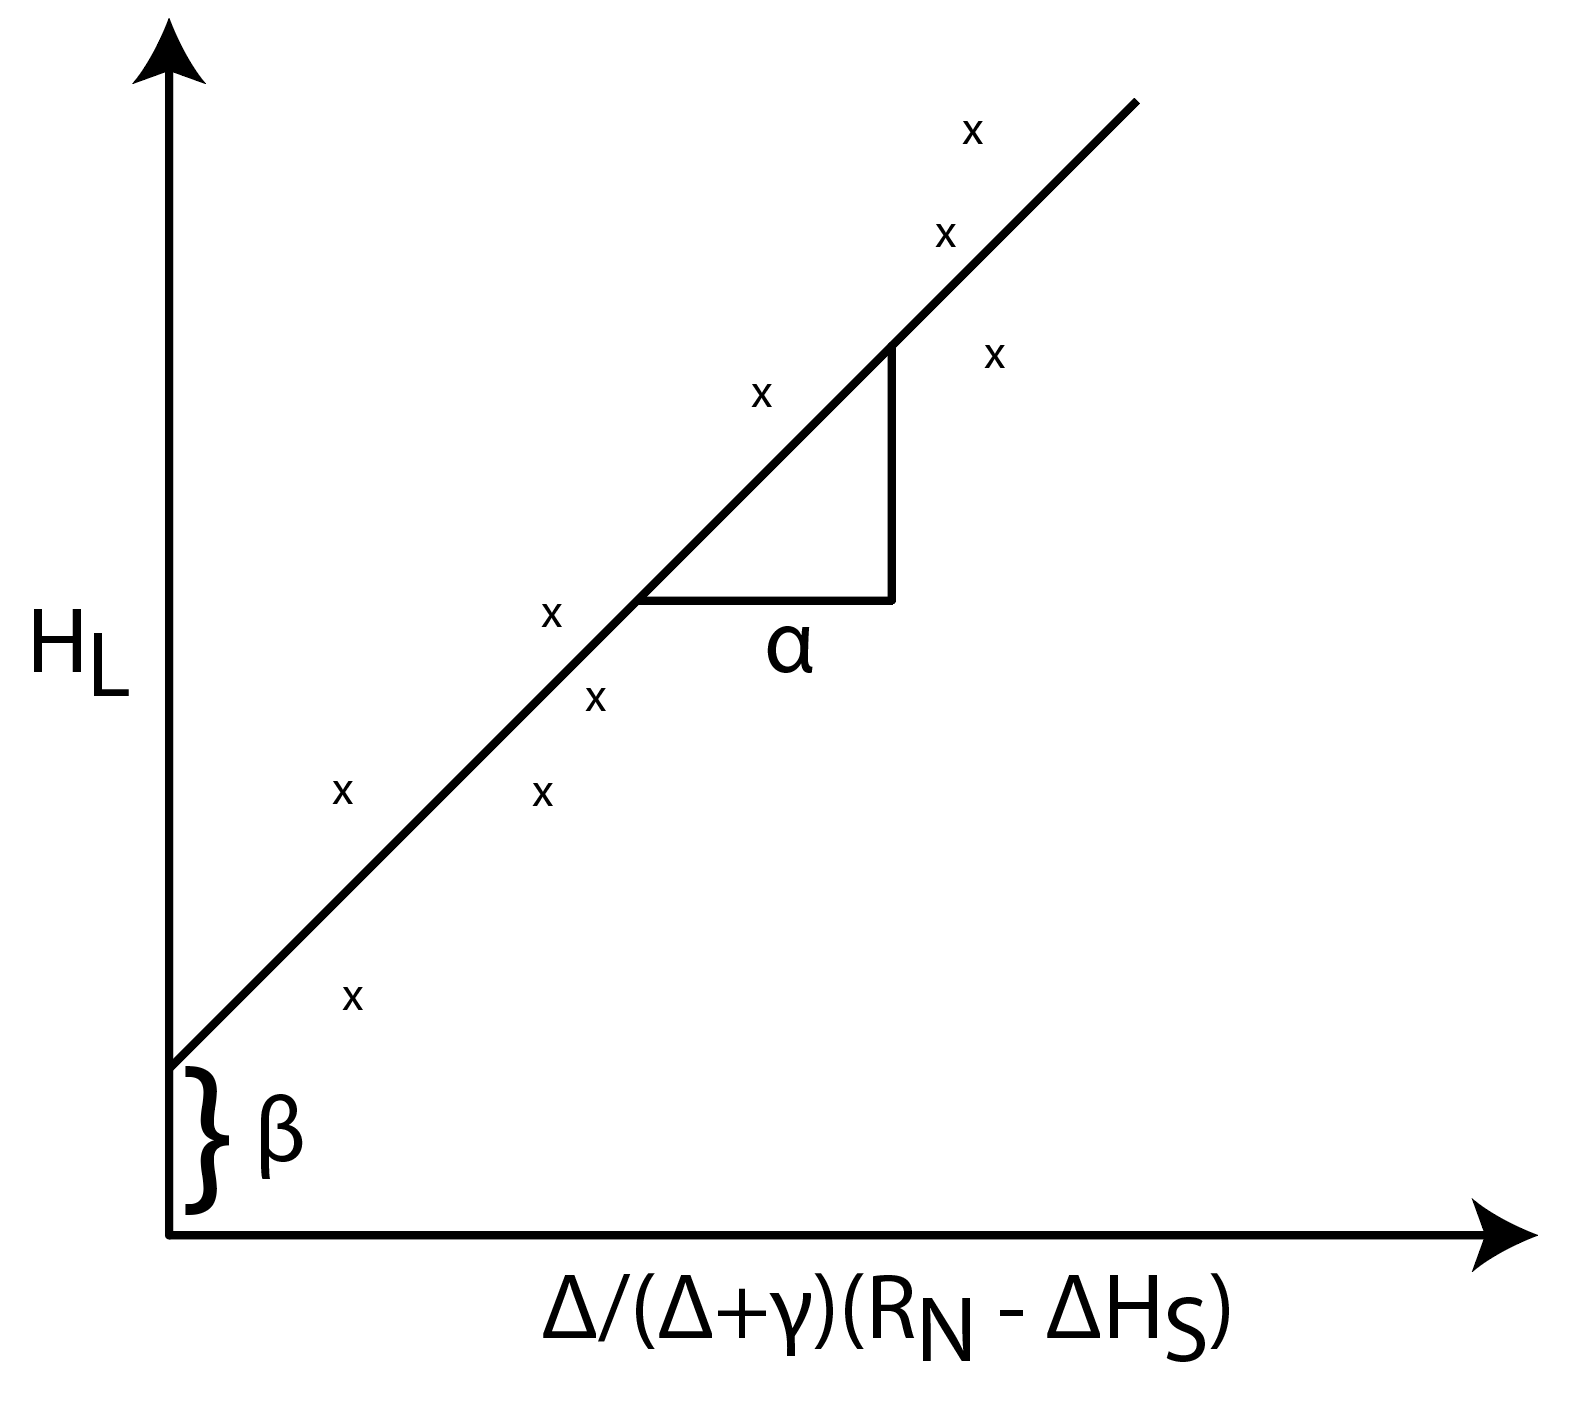
\includegraphics[width=0.6\textwidth]{fig8}
\end{figure}
\begin{itemize}
	\item $\alpha$ and $\beta$ are really just regression coefficients
	\item Recommended $\beta=20\ \watt\ \metre\rpsquared$ (Holtslag and van Ulden 1983)
	\item For urban surface, $\beta=3\ \watt\ \metre\rpsquared$ (Grimmond)
\end{itemize}

\end{frame}
%------------------------------------------------
\section{Static Stability} %
%------------------------------------------------
\framecard[colorred]{{\color{white}\Huge Static Stability}}
%------------------------------------------------
\subsection{Overview}
%------------------------------------------------
\begin{frame}{Static Stability}
Arya Chapter 5.3
\begin{itemize}
	\item Variations of temperature and humidity with height in PBL lead to density stratification
	\item As a consequence, an upward- or downward-moving air parcel will have a different density than its environment
	\item This leads to a buoyancy force that acts to accelerate/decelerate the vertical movement
	\item If the vertical movement is enhanced, the environment is \textbf{statically unstable}
	\item If the vertical movement is stopped, the environment is \textbf{statically stable}
	\item When the atmosphere exerts no buoyancy force, the environment is \textbf{neutral}
\end{itemize}
\end{frame}
%------------------------------------------------
\begin{frame}{Static Stability}
\begin{itemize}
	\item Using Archimedes principle (idea that there is a balance between pressure and the weight of an body at equilibrium), the buoyancy force is
	$$a_b=g\left(\frac{\rho - \rho_P}{\rho_P}\right)$$
	and using the equation of state for moist air
	$$a_b=g\left(\frac{T_v - T_{vp}}{T_v}\right)$$
	where the subscript $p$ refers to the parcel
\end{itemize}
\end{frame}

%------------------------------------------------
\subsection{Local Static Stability}
%------------------------------------------------
\begin{frame}{Local Static Stability}
\begin{itemize}
	\item We can approximate $a_b$ using the local gradient of virtual temperature
	$$a_b \approxeq -\frac{g}{T_v}\left(\frac{\partial T_v}{\partial z} + \Gamma\right)\Delta z = -\frac{g}{T_v}\frac{\partial \theta_v}{\partial z}\Delta z$$
	where
	$$\theta_v = T_v\left(\frac{1000}{p}\right)^\kappa$$
	is the virtual potential temperature, which allows for comparison of parcels with different pressures and moisture content - a very important parameter for stability determination
\end{itemize}
\end{frame}
%------------------------------------------------
\begin{frame}{Local Static Stability}
We define the static stability parameter $s$ as
$$s = \frac{g}{T_v}\left(\frac{\partial \theta_v}{\partial z}\right)$$
\begin{itemize}
	\item Unstable: $s<0$, $\partial \theta_v/\partial z < 0$, or $\partial T_v/\partial z < -\Gamma$
	\item Stable: $s>0$, $\partial \theta_v/\partial z > 0$, or $\partial T_v/\partial z > -\Gamma$
	\item Neutral: $s=0$, $\partial \theta_v/\partial z = 0$, or $\partial T_v/\partial z = -\Gamma$
\end{itemize}
\end{frame}
%------------------------------------------------
\begin{frame}{Local Static Stability}
Based on the virtual temperature gradient or lapse rate(LR), relative to the adiabatic lapse rate $\Gamma$, layers are characterized as
\begin{itemize}
	\item Superadiabatic: LR $> \Gamma$
	\item Adiabatic: LR $= \Gamma$
	\item Subadiabatic: LR $< \Gamma$
	\item Isothermal: LR $= 0$
	\item Inversion: LR $>0$
\end{itemize}
\end{frame}
%------------------------------------------------
\begin{frame}{Local Static Stability}
\begin{figure}
	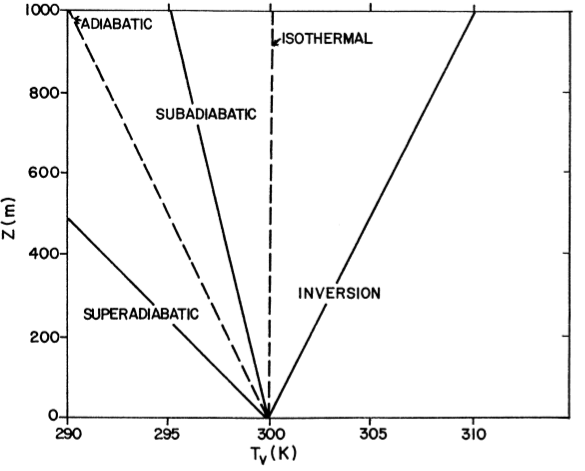
\includegraphics[width=0.9\textwidth]{fig9}
\end{figure}
\end{frame}
%------------------------------------------------
\begin{frame}{Local Static Stability}

\begin{itemize}
	\item The local view of static stability is limited and flawed
	\item This is especially true when used as a measure of turbulent mixing and diffusion
	\item The bulk of the CBL is a mixed layer ($\partial \theta_v /\partial z \approx 0$, or slightly positive)
	\item This would leave you to think this is a neutral or slightly stable layer according to local static stability theory
	\item However, the CBL has every attribute of an unstable layer: upward heat flux, strong mixing, large thickness
	\item Thus, $s$ is a poor metric for parcels that undergo large displacements from equilibrium - need a new idea not based on local gradients 
\end{itemize}
\end{frame}
%------------------------------------------------
\subsection{Mixed Layer}
%------------------------------------------------
\begin{frame}{Mixed Layer}
\begin{columns}[T]
    \begin{column}{.5\textwidth}
    \begin{minipage}[c][0.7\textheight][c]{\linewidth}
    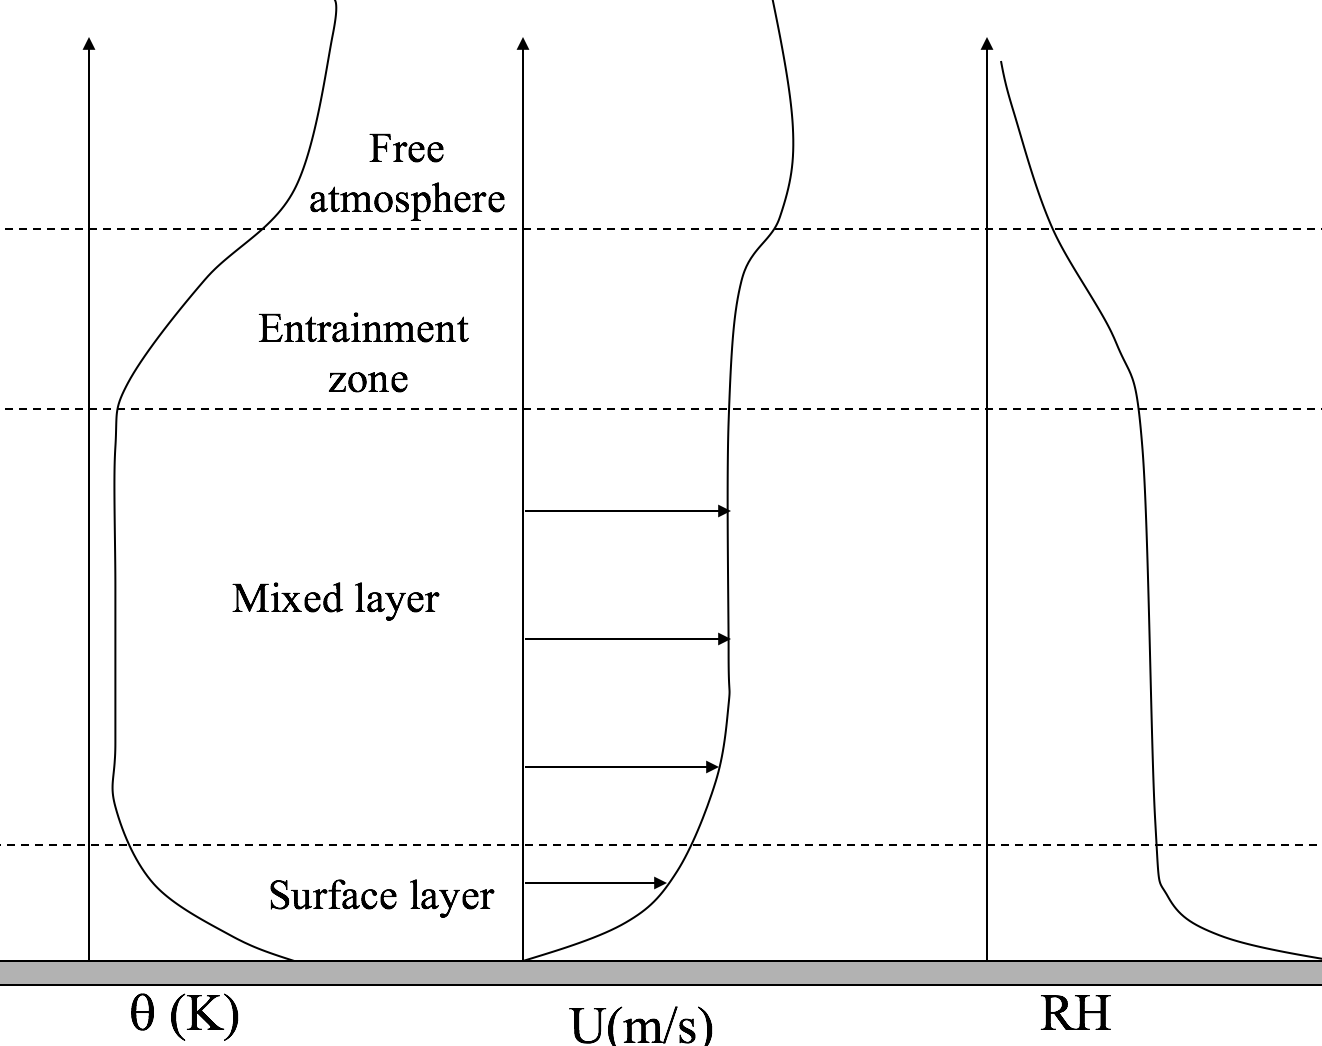
\includegraphics[width=1\textwidth]{fig12}\\
    \end{minipage}
    \end{column}
    \begin{column}{.6\textwidth}
    \begin{minipage}[c][0.6\textheight][c]{\linewidth}
   \begin{itemize}
   	\item layer where significant mixing occurs
   	\item most properties are constant
   	\end{itemize}
      \end{minipage}
    \end{column}
  \end{columns}
\end{frame}
%------------------------------------------------
\subsection{Inversion}
%------------------------------------------------
\begin{frame}{Mixed Layer}
\begin{columns}[T]
    \begin{column}{.5\textwidth}
    \begin{minipage}[c][0.7\textheight][c]{\linewidth}
    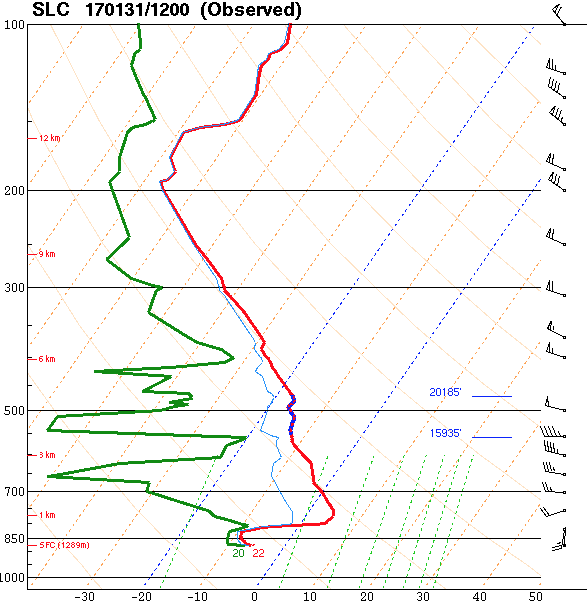
\includegraphics[width=1\textwidth]{fig13}\\
    \end{minipage}
    \end{column}
    \begin{column}{.6\textwidth}
    \begin{minipage}[c][0.6\textheight][c]{\linewidth}
   \begin{itemize}
   	\item $\theta_v$ increases with height (locally stable)
   	\item vertical mixing is inhibited, pollution can increase
   	\item examples: surface cooling in SL valley, cold pool,, warm sea breeze blowing over cool land
   	\end{itemize}
      \end{minipage}
    \end{column}
  \end{columns}
\end{frame}
%------------------------------------------------
\begin{frame}{Inversion}
\begin{figure}
	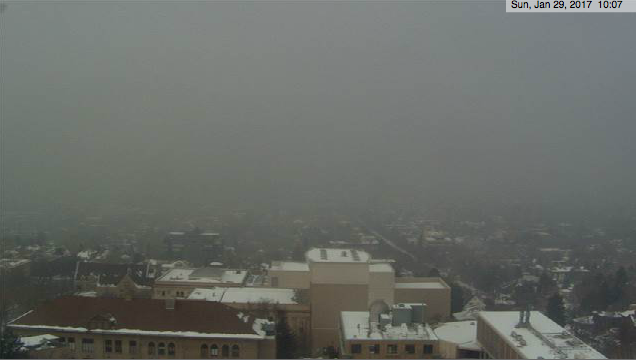
\includegraphics[width=\textwidth]{fig11}
\end{figure}
Yuck!
\end{frame}
%------------------------------------------------
\subsection{Non-Local Static Stability}
%------------------------------------------------
\begin{frame}{Non-Local Static Stability}
\begin{itemize}
	\item Enter non-local static stability (Stull 1991)
	\item Need soundings of environment over a deep layer up to place where vertical motions are irrelevant (strong inversion, tropopause)
	\item Stability is determined by displacing parcels from all possible locations in the domain
	\item Thus the stability is based on parcel buoyancy and not local lapse rates
	\item Parcel buoyancy at any level is determined by the difference in virtual temperatures of the parcel and environment
\end{itemize}
\end{frame}
%------------------------------------------------
\begin{frame}{Non-Local Static Stability}
\begin{itemize}
	\item Unstable: regions where parcels can enter and transit under their own buoyancy - note: parcels need not traverse the entire region
	\item Stable: regions of superadiabatic LR that are not unstable
	\item Neutral: regions of adiabatic lapse rates that are not unstable
	\item Unknown: Top or bottom portions of the sounding that appear stable or neutral, but do not end at a material surface (ground, inversion, etc) - because area above or below is unknown and could provide positive buoyancy
\end{itemize}
\end{frame}
%------------------------------------------------
\begin{frame}{Non-Local Static Stability}
\begin{figure}
	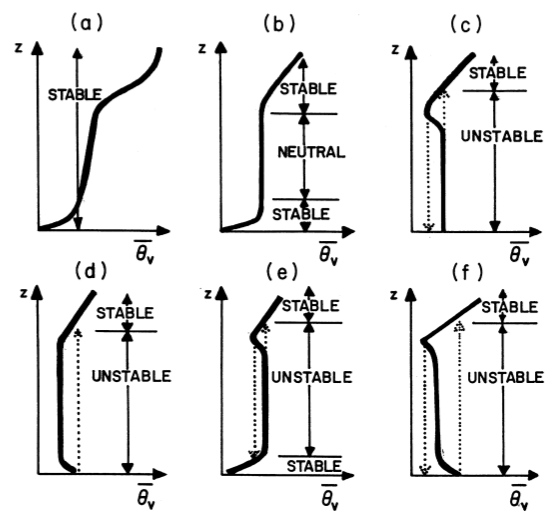
\includegraphics[width=0.8\textwidth]{fig10}
\end{figure}
\end{frame}

%------------------------------------------------
\end{document}

